\documentclass{pnastwo}
\usepackage[numbers,round,sort&compress]{natbib}
\usepackage{pnastwoF}
\usepackage{graphicx}
\usepackage{amssymb,amsfonts,amsmath}
\usepackage[american]{babel}
\usepackage{color}
\usepackage[section]{placeins}


\newcommand{\red}[1]{\textcolor{red}{#1}}
\renewcommand{\bibsection}{}


%% OPTIONAL MACRO DEFINITIONS
\def\s{\sigma}

% Fix wierd behavior which prevents table captions from appearing for
% tables in the body of the article
\makeatletter
\long\def\@makecaption#1#2{%
\ifx\@captype

\let\currtabcaption\relax
\gdef\currtabcaption{
\tabnumfont\relax #1. \tabtextfont\relax#2\par
\vskip\belowcaptionskip 
}
\else
 \vskip\abovecaptionskip
  \sbox\@tempboxa{\fignumfont#1.\figtextfont\hskip.5em\relax #2}%
  \ifdim \wd\@tempboxa >\hsize
\fignumfont\relax #1.\figtextfont\hskip.5em\relax#2\par
  \else
    \global \@minipagefalse
    \hb@xt@\hsize{\hfil\box\@tempboxa\hfil}%
  \fi
\fi
}
\makeatother

% And another fix.  PNAS class loses the label of floats unless they       
% were defined with the [h] option (so not really floats at all).  It      
% all comes down to wrong scope in the following routine which pushes      
% out the floats onto the page.  This is the fixed version:        
\makeatletter                                  
\def\DonormalEndcol{%                              
%% top float ==>                               
\ifx\toporbotfloat\xtopfloat%                          
%% figure ==>                                  
  \ifcaptypefig%                               
  \expandafter\gdef\csname topfloat\the\figandtabnumber\endcsname{%    
  \vbox{\vskip\PushOneColTopFig%                       
  \unvbox\csname figandtabbox\the\loopnum\endcsname%               
  \vskip\abovefigcaptionskip%                          
  \csname caption\the\loopnum\endcsname%                   
  \csname letteredcaption\the\loopnum\endcsname%               
  \csname continuedcaption\the\loopnum\endcsname%              
  \csname letteredcontcaption\the\loopnum\endcsname            
  \ifredefining%                               
  \csname label\the\loopnum\endcsname%                     
  \expandafter\gdef\csname topfloat\the\loopnum\endcsname{}\fi}%       
  \vskip\intextfloatskip%%                         
  \vskip-4pt %% probably an artifact of topskip??              
}%                                     
\else%                                     
%% plate ==>                                   
  \ifcaptypeplate%                             
  \expandafter\gdef\csname topfloat\the\figandtabnumber\endcsname{%    
  \vbox{\vskip\PushOneColTopFig%                       
  \unvbox\csname figandtabbox\the\loopnum\endcsname            
  \vskip\abovefigcaptionskip                           
  \csname caption\the\loopnum\endcsname                    
  \csname letteredcaption\the\loopnum\endcsname                
  \csname continuedcaption\the\loopnum\endcsname               
  \csname letteredcontcaption\the\loopnum\endcsname            
  \ifredefining                                
  \csname label\the\loopnum\endcsname                      
  \expandafter\gdef\csname topfloat\the\loopnum\endcsname{}\fi}        
  \vskip\intextfloatskip %%                            
  \vskip-4pt %% probably an artifact of topskip??              
}%                                     
\else% table ==>                               
 \expandafter\gdef\csname topfloat\the\figandtabnumber\endcsname{%     
 \vbox{\vskip\PushOneColTopTab %%                      
 \csname caption\the\loopnum\endcsname                     
  \csname letteredcaption\the\loopnum\endcsname                
  \csname continuedcaption\the\loopnum\endcsname               
  \csname letteredcontcaption\the\loopnum\endcsname            
  \vskip\captionskip                               
  \unvbox\csname figandtabbox\the\loopnum\endcsname            
\ifredefining                                  
\csname label\the\loopnum\endcsname                    
\expandafter\gdef\csname topfloat\the\loopnum\endcsname{}\fi           
}\vskip\intextfloatskip %% why don't we need this?             
\vskip-10pt}                                   
\fi\fi%                                    
%                                      
\else% bottom float                            
%                                      
\ifcaptypefig                                  
\expandafter\gdef\csname botfloat\the\figandtabnumber\endcsname{%      
\vskip\intextfloatskip                             
\vbox{\unvbox\csname figandtabbox\the\loopnum\endcsname            
\vskip\abovefigcaptionskip                         
  \csname caption\the\loopnum\endcsname                    
  \csname letteredcaption\the\loopnum\endcsname%               
  \csname continuedcaption\the\loopnum\endcsname%              
  \csname letteredcontcaption\the\loopnum\endcsname%               
\vskip\PushOneColBotFig%%                          
\ifredefining%                                 
\csname label\the\loopnum\endcsname                    
\expandafter\gdef\csname botfloat\the\loopnum\endcsname{}\fi}}%        
\else                                      
\ifcaptypeplate                                
\expandafter\gdef\csname botfloat\the\figandtabnumber\endcsname{%      
\vskip\intextfloatskip                             
\vbox{\unvbox\csname figandtabbox\the\loopnum\endcsname            
\vskip\abovefigcaptionskip                         
  \csname caption\the\loopnum\endcsname                    
  \csname letteredcaption\the\loopnum\endcsname%               
  \csname continuedcaption\the\loopnum\endcsname%              
  \csname letteredcontcaption\the\loopnum\endcsname%               
\vskip\PushOneColBotFig%%                          
\ifredefining%                                 
\csname label\the\loopnum\endcsname                    
\expandafter\gdef\csname botfloat\the\loopnum\endcsname{}\fi}}%        
  \else% TABLE                                 
\expandafter\gdef\csname botfloat\the\figandtabnumber\endcsname{%      
  \vskip\intextfloatskip                           
\vbox{\csname caption\the\loopnum\endcsname                
  \csname letteredcaption\the\loopnum\endcsname                
  \csname continuedcaption\the\loopnum\endcsname               
  \csname letteredcontcaption\the\loopnum\endcsname%               
  \vskip.5\intextfloatskip                         
  \unvbox\csname figandtabbox\the\loopnum\endcsname%               
\vskip\PushOneColBotTab                            
\ifredefining%                                 
\csname label\the\loopnum\endcsname                    
\expandafter\gdef\csname botfloat\the\loopnum\endcsname{}\fi}}%        
\fi\fi\fi}                                 
\makeatother                                   

%%%%%%%%%%%%
%% For PNAS Only:
\url{www.pnas.org/cgi/doi/10.1073/pnas.xxxxxxxxxx}
\copyrightyear{2008}
\issuedate{Issue Date}
\volume{Volume}
\issuenumber{Issue Number}
%\setcounter{page}{2687} %Set page number here if desired
%%%%%%%%%%%%

\begin{document}
\widowpenalty10000
\clubpenalty10000

\title{Developmental changes in the speed of social attention in early word learning}
\author{Daniel Yurovsky\affil{1}{Department of Psychology, Stanford University},
		Anna Wade\affil{2}{School of Medicine, University of California, San Francisco},
		Allison M Kraus\affil{1}{},
		Grace W. Gengoux\affil{3}{School of Medicine, Stanford University},
		Antonio Hardan\affil{3}{},
		\and Michael C. Frank\affil{1}{}}
\contributor{Submitted to Proceedings of the National Academy of Sciences of the United States of America}

\significancetext{The study of language development has historically focused on pinpointing children's earliest points of competence across domains. However, learning outside the laboratory is controlled by proficient use of the skills in these domains. While infants can follow social cues like eye-gaze in their first year, the speed and fidelity of this skill improves dramatically over the first five years. The problem of tracking social information is far from resolved for young infants; it remains a bottleneck on word learning for typically developing children into the preschool years and and does so for children with autism spectrum disorder as well. This work highlights the importance of studying not just origins, but also the developmental trajectories of higher-level cognitive processes.}

\maketitle

\begin{article}

\begin{abstract}
How do children learn new words so rapidly? One powerful source of information for discovering the meaning of a new word is the set of social cues (e.g. eye-gaze) provided by the speaker. Studies of children's use of social cues have generally focused on its emergence in early infancy. We show, however, that this early competence has a long developmental trajectory: Slow, continuous improvements in speed of social information processing occur over the course of the first five years of life. This developing ability to allocate social attention is a significant bottleneck on early word learning, predicting how well children learn new words over the same time period. Further, we show that the same bottleneck exists for children diagnosed with autism spectrum disorder, a disorder characterized by atypical social information processing. These results describe a route by which increases in social expertise can lead to changes in language learning ability and highlight the dependence of developmental outcomes on not just the existence of particular competencies, but on their proficient use in complex contexts.
\end{abstract}
\keywords{language acquisition | word learning | social cues | cognitive development}

%\subsection{Significance Statement}


\vspace{12 pt}

\dropcap{C}hildren's first years are a time of rapid change. One striking development is children's growing mastery of their native language: The typical child will go from saying her first word shortly before she turns one to producing 4000--5000 words by age five \citep{goulden1990}. The pace and breadth of this transformation have led to a search for early-available, precocious mechanisms that support children's language acquisition. Perhaps because of the fundamentally discrete nature of the units of language itself, much of this search has focused specifically on pinpointing the earliest emergence of these mechanisms \citep{lidz2003,bulf2011,shukla2011}. However, learning outside the laboratory is controlled not by early availability of these mechanisms, but by their proficient use in complex natural environments.	


%[but c.f.][]{fernald1998, port2005}. 


 % Reviews of language development are often a list of milestones: e.g., infants acquire the ability to use sequential statistics to segment speech at 8 months \citep{saffran1996}, begin to use co-occurrence statistics to learn word-object mappings at 12 months \citep{smith2008}, and begin to use syntax to infer the meanings around 24 months \citep{gertner2006}. New exciting work then is often a demonstration of some competence earlier than previously observed \citep{bergelson2012}.

Here we take as a case study children's use of social information to infer the meanings of new words. Though even the earliest vocabulary contains words belonging to many grammatical categories, a large proportion are concrete nouns \citep{bates1994}. While acquiring a fully adult-like meaning for any of these nouns likely unfolds over multiple encounters, the very first problem a child faces when hearing a new word is referential uncertainty: Does the word refer to something in the current situation, and if so, what \citep{carey1978, yu2007, frank2009}? A powerful source of information for resolving this uncertainty is available in the social cues provided by the speaker; knowing where a speaker is looking is helpful for knowing what they are communicating about. Consequently, a large body of research documents and explores young infants' ability to track a speaker's social cues and use them to infer the target of her reference \citep[e.g.,][]{scaife1975, baldwin1993, hollich2000, senju2008}.

Much of the work in this research program has focused on discovering the earliest point of infants' competence in using social information. Underlying this focus is an implicit assumption that once the general ability to use social cues is demonstrated, children's proficiency with processing these cues is relatively high \citep[e.g.][]{corkum1998, brooks2005, csibra2009}. This research strategy stands in contrast to work in domains like visual and motor development, or even spoken word recognition, in which researchers have sought to measure continuous improvement in children's abilities as they develop \citep{sokol1978, banks1980, forssberg1991, thelen1995,fernald1998}. In these domains, continuous, quantitative changes can have as much impact on an infants' interaction with the world as qualitative changes \cite{adolph2015}. For example, the transition from crawling to walking leads to some advantages in children's ability to explore. However, infants' initial mobility after this transition is nowhere near as great as what they will achieve with another few months of practice \cite{adolph2012}. The emergence of the behavior is only the beginning.

Our goal in this article is to follow this same developmental strategy---of measuring continuous improvement---to understand how children use social information to learn new words. Using social information to resolve referential uncertainty is a highly time-sensitive process of continuous re-allocation of attention between the speaker and the objects in the context. Indeed, recent work has shown that rapid gaze-following occurs relatively rarely in natural parent-child interactions, and is difficult even for older children and adults under some circumstances \citep{loomis2008, vida2012, yu2013}. Thus, we hypothesize that competence in gaze following is not enough: the referential uncertainty problem should remain a problem in proportion to a children's developing ability to control their attention, process auditory and visual information, and hold the information in memory \citep{dempster1981, kail1991, gathercole2004}.

\begin{figure*}
        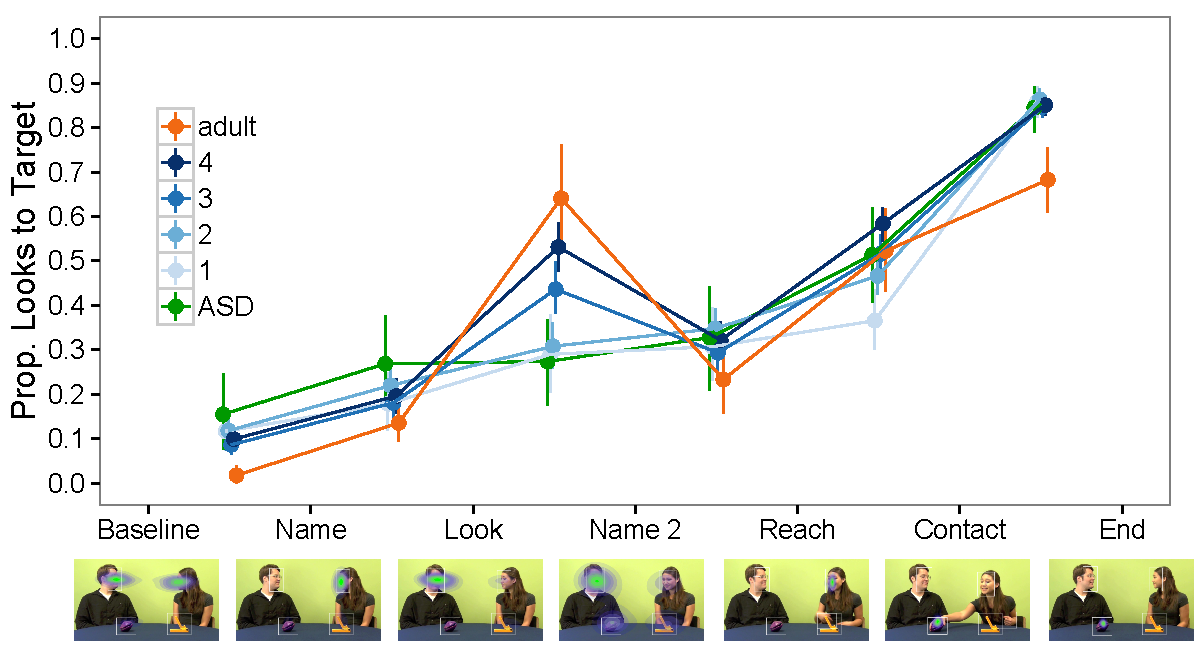
\includegraphics[width=.95\textwidth]{figures/bronto_all.pdf}
	\caption{\label{fig:reflook_learning} (bottom) Looking to Target vs. Competitor objects during the learning portion of Experiments 1 (typically-developing children and adults) and 2 (children with ASD), plotted by phase of the naming event. Points show means and error bars show 95\% confidence interval across participants; points are offset on the horizontal to avoid overplotting. Colors indicate age in years for typically developing children. (bottom) Example frames from the first word learning dialogue in Experiment 1. Each image shows the regions of interest used for later analysis (white boxes) and a heat map of the distribution of all participants' points of gaze over time (brighter colors indicate more fixation; scale is constant across frames)}
\end{figure*}

In three experiments, we test this hypothesis, showing that the developing ability to rapidly direct attention in social interactions is a bottleneck on children's word learning. We constructed videos that used novel words in a series of naturalistic object-focused dialogues and monologues. These videos were designed to be sufficiently difficult in their structure that in-the-moment disambiguation would pose a significant challenge to young learners, yet sufficiently simple that the repeated co-occurrence of novel words and the objects they label could allow for successful word learning. We measured children's eye-movements during viewing as an index of their online inferences about the current conversational referent, and then tested their retention of the words they learned via a series of forced-choice test trials. These rich time-course data allowed us to test two predictions: (1) although infants show measurable competence in social information processing, this ability has a long developmental trajectory, and (2) this developing ability is linked to language learning: children who successfully attend to speakers' social cues learn and retain the novel words they hear the speakers produce.

In Experiment 1, we measured developmental changes in social information processing and used these to predict word learning in typically developing children. In Experiment 2, we tested a sample of children diagnosed with autism spectrum disorder in the same paradigm as Experiment 1. We showed that social attention was a bottleneck on their learning from these videos in the same way as for the typically developing children. In Experiment 3, we manipulated the timing of social information directly to test the causal role of fast social attention, again in typically developing children. In all three studies, we recruited children across a broad age range, giving us the power to see continuous changes in both social attention and novel word learning.

\section{Experiment 1: Social Attention and Word Learning}

Experiment 1 was designed to estimate the developmental trajectory of children's online social information processing in complex interactions, and to ask whether this processing has downstream consequences for word learning. The experiment consisted of two sections: Learning and Test. During the learning section, participants watched a series of dialogues and monologues in which actors introduced and discussed two novel objects and two familiar objects. Each video contained two naming sequences (pictured in Fig.~\ref{fig:reflook_learning}, bottom); these sequences were broken into a series of phases during which the speaker named, looked at, named again, and reached for a particular object, allowing for the separate measurement of name-, gaze-, and reaching-related changes of attention.

We first measured the proportion of time that participants spent looking at the target referent during the naming sequences (Fig. ~\ref{fig:reflook_learning}, top). We analyzed these gaze trajectories by fitting a mixed-effects model predicting looking at the target from naming phase, age, and their interaction. Children increased their looking to the target object over the course of learning trials, with above-baseline looks to the target in all phases after the second naming. For all age groups, looking to the target toy reached nearly 100\% by the end of these events---after the speaker had made contact with the toy ($\beta_{name2-reach} = .18$, $t = 3.73$, $p < .001$; $\beta_{reach-contact} = .13$, $t = 2.56$, $p < .01$; $\beta_{contact-end} = .75$, $t = 15.8$, $p < .001$). The effect of age was not significant, but there was a significant interaction between age and phase---older children looked significantly more in the phases after the speaker's initial look and initial reach ($\beta_{look-name2} = .11$, $t = 7.66$, $p < .001$ ; $\beta_{reach-contact} = .08$, $t = 5.83$, $p < .001$). While the youngest children were only occasionally able to follow the speaker's social cues, older children and adults were much more consistent. Thus, the ability to process social information quickly and reliably in a naturalistic conversation improves markedly over the course of the first five years, and even further into adulthood.

\begin{figure}[tb]
	\center{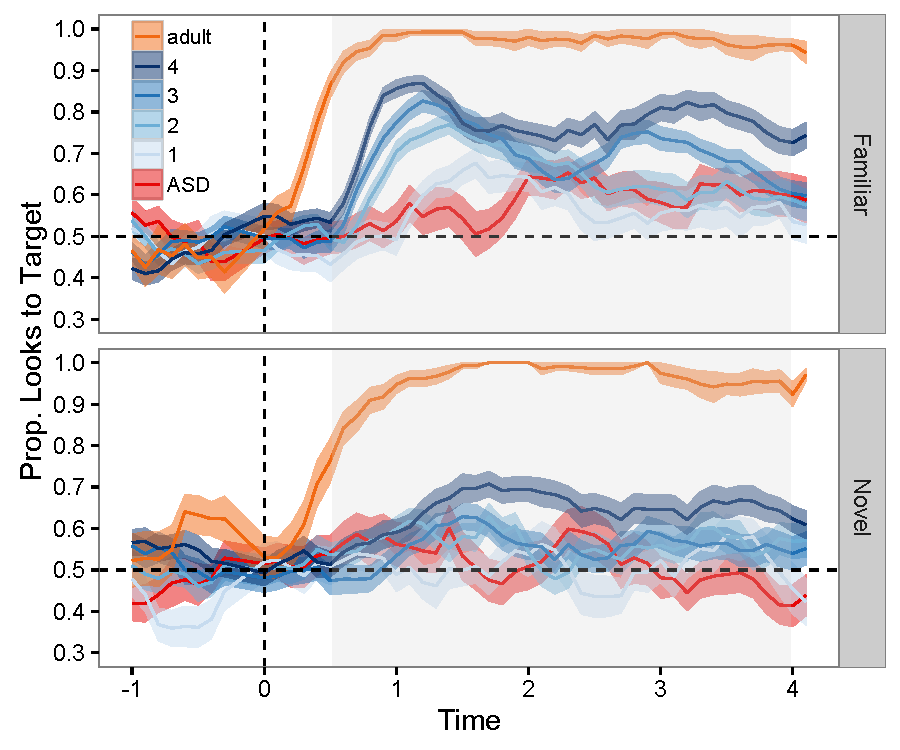
\includegraphics[width=.475\textwidth]{figures/reflook_timecourse.pdf}}
	\caption{\label{fig:reflook_timecourse}Children's and adults' looks to the Target and Competitor objects over the course of Test trials for typically developing children and adults (Experiment 1) and children with ASD (Experiment 2). Lines show age-group means, and shaded regions show standard errors of these means. The light gray rectangle shows the window over which looking proportions were computed for subsequent statistical analyses.}
\end{figure}

After watching these naming events, children's learning of the novel words was tested using the looking-while-listening procedure \citep{fernald1998, fernald2008}. On Test trials, children saw two toys on the screen and heard a voice asking them to find the target toy. On some trials, the target was a one of the Novel toys from the Learning trials (e.g. ``fep''). On other trials, the target was a familiar object whose label is typically in the comprehension vocabularies of young children (e.g. ``dog''). These Familiar trials allowed us to measure children's language comprehension more generally (Fig.~\ref{fig:reflook_timecourse}). Children in all age groups successfully looked at Familiar referents at above chance levels (smallest $\mu_{1-year} = .57$, $t(28) = 4.05$, $p < .001$), and all but the one-year-olds reliably learned the Novel words (smallest $\mu_{2-year} = .56$, $t(51) = 3.96$, $p < .001$). A linear model showed that children performed better on Test trials over development ($\beta_{age} = .07$, $z = 7.87$, $p < .001$), and that the effect of age was greater for Familiar than Novel trials ($\beta_{age * novel} = -.029$, $z = -2.40$, $p < .05$, Fig.~\ref{fig:reflook_timecourse})

Thus, older children learned more from the same naming events. These children also more quickly followed the speakers' social gaze and reaches, and more quickly processed Familiar words. All of these factors were independently, significantly correlated with learning ($r_{age}(196) = .29$, $p < .001$); $r_{familiar}(196) = .20$, $p < .01$; $r_{look-name2}(189) = .34$, $p < .001$; $r_{reach-contact}(191) = .17$, $p < .05$). Which of these factors was most responsible for improvements in learning? To answer this question, we fit a linear regression, predicting learning from age, familiar word processing, and looking to the target in the two relevant windows---after the look, and after the reach. Only looking to the target referent following the initial look reached significance ($\beta_{look-name2} = .14$, $z = 3.26$, $p < .01$), although age was marginal ($\beta_{age} = .02$, $z = 1.60$, $p = .11$). Because these predictors were all correlated, we also fit this same model after first residualizing out the effect of age on learning. In this model, gaze-following still remained highly significant ($\beta_{look-name2} = .11$, $z = 2.95$, $p < .01$).

Children who were unable to follow the speaker's social cues to determine the toy that was the topic of conversation were unable to learn that it was associated with the novel word in the discourse. Thus, age-related improvements in social attention, whatever their cause, play a powerful role in determining how much children learn from naming events throughout early childhood. The early emergence of this important competence is no guarantee of its proficient use in natural contexts.

\section{Experiment 2: Social Attention in Children with Autism}

The naming events in Experiment 1 contained information sufficient to infer the meanings of the novel words at two timescales. First, children could learn the meanings within the interactions by following the informative social cues. Second, children could learn these meanings across the interactions by using co-occurrence statistics between the words and objects \citep{smith2008}. In our data, typically developing children's social information processing predicted a considerable part of the variance in their word learning, suggesting that they may have learned largely via the social cues. Do children with atypical trajectories of social development rely more on co-occurrence statistics instead?

Children on the autism spectrum are one population whose strategy might be expected to differ. Deficits in social information processing in children with autism spectrum disorders have profound consequences for language learning \cite{baron-cohen1997,leekam1998}. One possibility is that because of these deficits, if children with autism learn in our paradigm, it would be due to cross-situational statistical learning. Another possibility however is that their social information processing impairments lie on a continuum with other, less extreme changes in social information processing that are still impactful for language learning \cite{brooks2005}. On this second account, their social information processing should be related to their learning outcomes, just as in typically-developing children.

To address this question, we tested a group of 40 2--8-year-old children diagnosed with autism spectrum disorder (ASD). These children did indeed process social information less efficiently---following the speaker's gaze no better than the youngest children in our sample (Fig.~\ref{fig:reflook_learning}). They also learned the Novel words, and attended to the referents of Familiar words at approximately the same levels (Fig.~\ref{fig:reflook_timecourse}). However, while age was uncorrelated with Novel word learning for the children with ASD ($r(28) = .11$, $p =.57$), following the speaker's social gaze was highly correlated with Novel word learning ($r(21) = .58$, $p <.01$), just as in the typically developing sample (Fig.~\ref{fig:corr_plot}). We again fit a linear regression, predicting Novel word learning from age, Familiar word processing, and looking to the Target in the two relevant windows---after the look, and after the reach. This model showed significant effects of Familiar word processing ($\beta_{familiar} = .51$, $z = 2.48$, $p < . 05$) and gaze following ($\beta_{look-name2} = .25$, $z = 3.06$, $p < .01$).

Thus, social information processing is a bottleneck on word learning for children with autism spectrum disorder, just as it is for typically developing children. Although as a group these children's looking behavior during learning trials was different from the looking behavior of their typically developing peers, children with ASD who successfully learned the Novel words did so by following social cues.

\begin{figure}[tb]
	\center{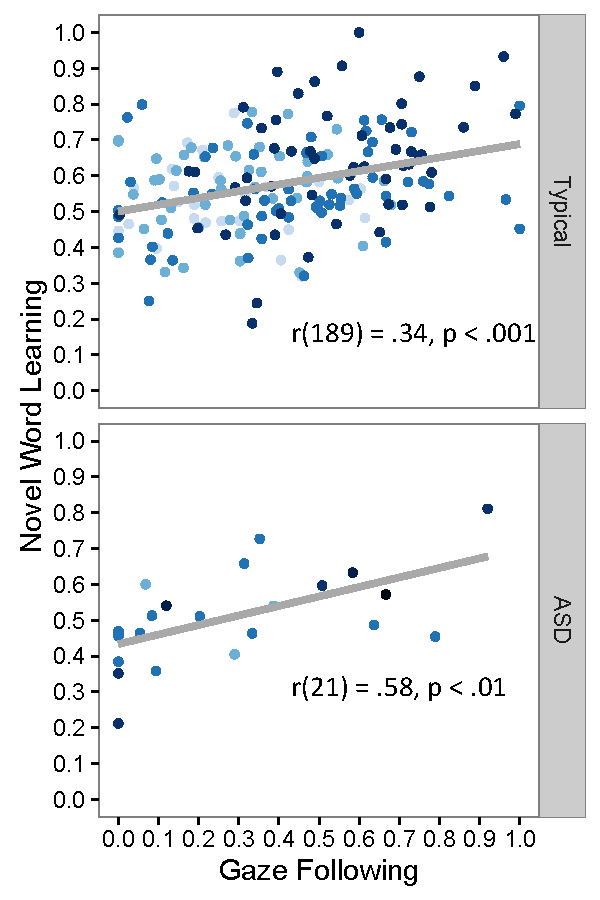
\includegraphics[width=.4\textwidth]{figures/corr_plot.pdf}}
	\caption{\label{fig:corr_plot}Correlations between gaze-following on Learning trials and accuracy on Novel Test trials for typically developing children in Experiment 1 and children with autism spectrum disorder (ASD) in Experiment 2. Darker colored points indicate older children.}
	
\end{figure}

\section{Experiment 3: Varying Demands on Social Attention}

The naming events in Experiments 1 and 2 provided children with a number of informative cues to the referents of the novel words: social gaze, speaker's manual interaction, and also cross-situational co-occurrence statistics. Our analyses showed that fast processing of social gaze was a strong predictor of children's ultimate word learning. In Experiment 3, we tested this prediction directly by manipulating the accessibility of the social cue.

In Experiment 3, the two Novel words were introduced in two different kinds of naming events. In Extended Hold events, the speaker made contact with and manipulated the Target toy for the duration of the naming event, providing an extended cue to the target of her referential intention. In contrast, in Brief Look events, the speaker only provided punctate gaze information, looking to the target of her referential utterance briefly after naming it and then looking forward towards the camera for the remainder of the naming event. On the basis of the results from Experiments 1 and 2, we predicted that Extended Hold trials would show less developmental differentiation in social attention and be easier to learn from. In contrast, we predicted that following the Brief Look would require rapid reallocation of social attention, and thus that older children would succeed in following the speaker's gaze while younger children failed. Further, we predicted that this difference in gaze-following would produce down-stream differences in learning.

As predicted, on Extended Hold trials, children spent a large proportion of the naming events looking at the Target across age groups ($\mu_{1-year} = .57$, $\mu_{2-year} = .60$, $\mu_{3-year} = .63$, $\mu_{4-year} = .60$), and age was not significantly correlated with looking behavior ($r(290) = .08, p = .15$). In contrast, children spent a much lower proportion of Brief Look events looking at the Target, and this proportion increased across age ($\mu_{1-year} = .09$, $\mu_{2-year} = .09$, $\mu_{3-year} = .16$, $\mu_{4-year} = .17$; $r(288) = .27$, $p  < .001$).

As before, children in all age groups showed evidence of processing Familiar words at above chance levels (smallest $\mu_{1-year} = .59$, $t(63) = 5.09$, $p < .001$). Children two-years-old and older showed evidence of learning from the Extended Hold trials (smallest $\mu_{2-year} = .63$, $t(66) = 5.43$, $p < .001$), but only the 3- and 4-year-olds learned from the Brief Look trials (smallest $\mu_{3-year} = .58$, $t(68) = 3.66$, $p < .001$). To confirm these analyses, we fit a mixed effects model predicting looking at the correct referent on Test trials from children's age and the trial type. Children improved significantly over development ($\beta_{age} = .08$, $t = 19.34$, $p < . 001$). Children's Test trial performance also varied significantly across trial types. Relative to novel words encountered in Extended Hold events, children performed better on Familiar words($\beta_{Familiar} = .09$, $t = 6.64$, $p < . 001$) and worse on Novel words encountered in Brief Look events ($\beta_{Brief Look} = -.09$, $t = -6.48$, $p < . 001$).

To succeed on Test trials, children needed to succeed at two tasks: first, process social information available in learning trials to disambiguate naming events and discover the speaker's intended referent; and second, process the language they heard at test, and use it to retrieve the correct mapping between the Novel word and the target referent. The Extended Hold events were designed to reduce demand on children's online social information processing, rendering language processing and memory retrieval the only bottlenecks on Test trials.

We leveraged this relationship to perform an additional test of our primary hypothesis: We fit a mixed effects model predicting children's Novel Test performance from their age, their Familiar word processing, and the naming event type (Extended Hold vs. Brief Look), as well as the interaction of Familiar word processing and naming event type. This model showed a significant effect of age ($\beta_{age} = .05$, $t = 4.83$, $p < . 001$), as well as a significant interaction between Familiar word processing and naming event type($\beta_{Extended Hold * Familiar} = .21$, $t = 3.47$, $p < . 001$). Familiar word processing was a better predictor of children's success on Extended Hold trials, where language processing---not social information processing---was the primary bottleneck.

Together, these results demonstrate the powerful role of fast social information processing in early word learning. All of the children were able to follow the speaker's social cues when they Extended over the entire naming event, and this supported their learning. In contrast, only the older children were able to follow the Brief Look, and only they were consequently able to learn from it.


\begin{figure}[tb]
	\center{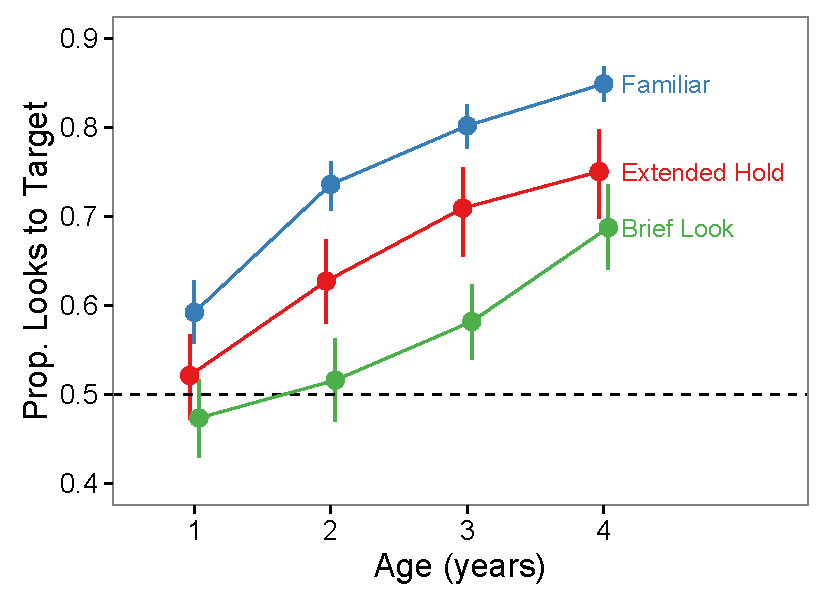
\includegraphics[width=.475\textwidth]{figures/soc_word_test.pdf}}
	\caption{\label{fig:soc_word_test}Test trial performance in Experiment 3 for the Familiar words, as well as for Novel words that appeared in Brief Look and in Extended Hold learning events. Error bars show 95\% confidence intervals computed by non-parametric bootstrap; points are offset on the horizontal to avoid overplotting.}
\end{figure}


\section{Discussion}

The early emergence of children's linguistic and communicative capacities is extraordinary. Infants show evidence of following social cues and understanding the communicative function of language by 6 months of age \citep{senju2008, vouloumanos2014}. By the same early age, infants can learn about the structure of their languages by tracking the distributional properties of the speech they hear, and even appear to have at least nascent meanings for some words \citep{thiessen2003, bergelson2012}. A large body of research in developmental psychology has taken the early emergence of these abilities as evidence for expertise, implicitly or explicitly endorsing the idea that children learn language quickly because they are expert social and distributional information processors.

But early competence is not enough to produce rapid learning. Children must also be able to \emph{perform} these abilities rapidly and robustly in complex real-world settings. We show that this performance has a long developmental trajectory: social information processing improves dramatically over the first five years of life. While one-year-olds were able to follow social gaze occasionally in our experiments, this level of performance did not translate into novel word learning. And even four-year-olds, whose performance was much better, still did not shift their social attention as flexibly as adults.

This social information processing bottleneck also characterized the learning of our sample of children with autism spectrum disorder. Autism is a complex and heterogeneous disorder, affecting different children to different degrees, and in different ways. Nonetheless, one of the core deficits appears to be a disorder of social information processing. This deficit was manifest in our data---children with autism spectrum disorder performed substantially lower than typically developing children in following social cues and learning new words. But critically, variability in social information processing among these children predicted variability in learning just as with the typically developing children.  We take this as evidence for generality of social information processing to word learning: Successful learners were successful in the same way.

Although these experiments provide evidence for pronounced and continual improvement in children's social information processing, they leave open the question of what is responsible for these changes. One possibility is that these changes in social attention are caused by domain-general developmental changes in attentional control more broadly \citep{rueda2005,smith2013}. Alternatively, these children could be refining their domain-specific representations of the visual and temporal structure of conversations, producing better predictions about where speakers will look and reach next \citep{acheson2009,krogh-jespersen2015}. In either case, we propose that these changes may play a powerful role in explaining the rapidly accelerating pace of children's language learning. Indeed, while much has been made of the changes in word learning that occur in the first and second years, the rate at which children learn words continues to increase over the third, fourth, and fifth years \citep{bloom2000}.

Of course, these experiments are not without their limitations. Although we endeavored to recruit a large and developmentally diverse set of participants, the primary data in Experiments 1 and 2 are correlational in nature. Experiment 3 was designed to causally manipulate social information, providing stronger evidence for the correlation observed in the Experiments 1 and 2. In addition, to minimize variability in stimulus presentation across children, we used a set of fixed video stimuli. It is possible that the use of videos actually underestimates children's social information processing and learning \citep{anderson2005}. However, more recent work has shown that the ``video deficit'' in learning is ameliorated when children observe the kinds of reciprocal interaction that characterize the dialogues in Experiment 1  \citep{odoherty2011}.

Finally, while we endeavored to construct naturalistic stimuli that represent the kinds of interactions characteristic of children's language learning environments, they are far from exhaustive. In order to minimize measurement noise, we artificially fixed the learning environment for each child, but the natural learning environment varies considerably across children and across development. Indeed, children who receive more high-quality language input learn more language \citep{weisleder2013}. But rapid language learning may require more than the right input; children might need the right input at the right time.

If infants' social information processing performance is so poor, why do they learn words so rapidly? One intriguing possibility is that parents may tune their visual and linguistic input to their children's developing social information processing skills \citep{snow1972,gogate2000,brand2002}. That is, caregivers may not use Brief Looks to indicate their referents for young children, but instead use Extended Holds (Experiment 3). Perhaps rapid early word learning is not a result of early expertise per se, but instead emerges from the interaction between children's developing processing skills and their caregivers' coordinated linguistic and social input.

\begin{materials}

\subsection{Participants} Data from typically-developing children were collected at the San Jose Children's Discovery Museum, where parents and their children were invited to participate in an experiment investigating children's early word learning after providing informed consent. In Experiment 1, we collected both demographic and eye-tracking data from 349 children in the target age range, of whom 113 were excluded from the final sample for one or more of the following reasons: unacceptable eye-tracker calibration or data ({\small$N=49$}), atypical developmental trajectories ({\small$N=30$}), and less than 75\% parent-reported exposure to English ({\small$N=41$}). Our final sample included 238 children (42 1-year-olds (21 girls); 66 2-year-olds (32 girls); 74 3-year-olds (36 girls); and 56 4-year-olds (30 girls)). In Experiment 3, we collected demographic and eye-tracking data from 425 children in the target age range, of whom 201 were excluded from the final sample for one or more of the following reasons: unacceptable eye-tracker calibration or data ({\small$N=96$}), atypical developmental trajectories ({\small$N=36$}), and less than 75\% parent-reported exposure to English ({\small$N=48$}). Our final sample included 224 children, ages 1---5 (60 1-year-olds (24 girls); 57 2-year-olds (29 girls); 51 3-year-olds (25 girls); and 50 4-year-olds (24 girls)).

Data from children with ASD were collected at Stanford University. Children with ASD and their siblings were primarily recruited through the Autism and Developmental Disorders Research Registry, and by flyers posted in the Autism and Developmental Disorders Clinic. Children with a diagnostic history of ASD underwent a comprehensive diagnostic evaluation to determine the accuracy of the previous diagnosis based on DSM-5 criteria, which was confirmed with research diagnostic methods. These diagnostic methods included the ADI-R \citep{lord1994,le-couter1989} and the Autism Diagnostic Observation Schedule -- Generic (ADOS-G) \citep{lord1999,lord2000}. Exclusion criteria included: 1) a genetic, metabolic, or infectious etiology for ASD on the basis of medical history, neurological history, and available laboratory testing for inborn errors of metabolism and chromosomal analysis; and 2) a DSM-5 diagnosis of any severe mental disorder such as schizophrenia and bipolar disorder. We collected demographic and eye-tracking data from 51 1--7-year old-children, of whom 10 were excluded for unacceptable eye-tracker calibration. The final sample comprised 41 children ({\small$M_{age}$} = 4.22-years, range = (2.24--7.97-years), 4 girls).

Adult participants in Experiment 1 were 17 Stanford undergraduate students who participated in exchange for course credit. Informed consent was obtained from parents of all children, and from all adult participants, before experiments began.

\subsection{Stimulus and Design} After an initial eye-tracker calibration phase, children and adults in both experiments watched a $\sim$6 minute video. Each video presented two kinds of trials. Learning trials consisted of videos in which speakers seated at a table with two toys provided social cues and labeled one of the toys. Test trials showed pictures of two objects on a black background while a voice asked the participant to look at one of them \citep[as in][]{fernald1998}.

In addition, each video included a re-calibration stimulus which participants saw a small, brightly colored stimulus move around the screen. These phases of the videos were used to correct the calibrations estimated at the beginning of the experiment \citep[see][]{frank2012}. Finally, videos contained a small number of filler trials in which participants saw engaging pictures or videos designed to keep maintain their attention for the duration of the video.

Learning trials varied across the Experiments. In Experiment 1 and 2, these learning trials consisted of two dialogues in which two speakers sat at a table together, and one referred to each of the two novel toys whose names were taught in the experiment (``toma'' and ``fep''). The other two learning trials were monologues in which one of the speakers sat at a table alone, with one of the novel toys and one familiar toy and referred to each in turn. Each naming event consisted of six events: first a naming phrase, then a look at the object accompanied by a comment, a second naming, a reach for the object, and finally a demonstration of the object's function accompanied by a third naming. Each novel object was named nine times in total over the course of the video. Participants watched all of the learning trials before they began the test trials. Eight of these test trials tested familiar objects (e.g. dog/car or lamp/carrot); the other eight paired the two novel objects. Naming phrases were of the form ``Look at the [car/fep]! Do you see it?'' and were spoken by the actors in the video.

In Experiment 3, we simplified the learning trials. All naming sequences were monologues and both toys on the table were novel.  Four of the naming sequences were Extended Hold trials, in which the speaker reached for and interacted with one of the two toys while describing its function and producing its name three times. The other four were Brief Look trials in which the speaker produced the same kind of description but indicated the target toy only with a brief look after first producing its label. Brief Look and Extended Hold trials used a distinct but consistent set of two toys, and the same toy was consistently either the target or the competitor on each trial type. Because children in Experiment 1 sometimes lost interest in these videos before reaching the test trials, in Experiment 3 test trials were interspersed with learning trials so that at least some test data could be acquired from each child. In total, Experiment 3 contained 20 test trials. Eight of these test familiar objects as in Experiments 1 and 2. Eight paired the named objects from the learning trials against their foils from the learning trials, four for the object named in Brief Look trials, and four for the object named in Extended Hold trials. The remaining four test trials paired the two named objects against each other, with children being asked to find each two times.

\subsection{Data Analysis}

In all experiments, raw gaze data went through several transformations before statistical tests were computed. First to ensure appropriate precision in region-of-interest analyses, infants' calibrations were corrected and verified via robust regression \citep[described in][]{frank2012}, and calibration corrections were assessed by two independent coders ({\small$\kappa_{Exp1} = .8$}, {\small$\kappa_{Exp2} = .87$}, {\small$\kappa_{Exp3} = .76$}). Children whose calibrations could not be verified and corrected were excluded from further analyses.

Second, all analyses were performed use an Area of Interest (AOI) approach. On learning trials, AOIs were hand-coded frame-by-frame for each of the speakers' faces and for the two on-screen objects. On test trials, these AOIs corresponded to the static on-screen positions of the two alternatives. To use standard statistical analyses, we transformed the timecourse data to proportions of looking within relevant windows. On test trials the start of this window was set to 500ms after the point of disambiguation---the onset of the target label. The end of the window was set to the length of the shortest test trial for accurate averaging. This was 4s for Experiments 1 and 2, and 4.5s for Experiment 3. These windows were chosen to give all children sufficient time to process the label, and to maximize signal (see Fig.~\ref{fig:reflook_timecourse}).

In Experiments 1 and 2, learning trials contained six distinct phases (Fig.~\ref{fig:reflook_learning}): a baseline period of exactly 2 s, name 1 to look ({\small$M$ = 1.7s}), look to name 2 ({\small$M$ = 2s}), name 2 to initiation of reach ({\small$M$= 4.8s}), initiation of reach to point of contact ({\small$M = .8s$}), and after contact with the object ({\small$M$ = 1s}). Proportion of looks to the target AOI were computed in each of these windows. In Experiment 3, learning trials were designed to separate demands on social attention across rather than within trials. In Experiment 3 we computed proportion of looking of the entirety of learning trials.

Due to occasional bouts of inattention, eye-gaze data were not available for all children during all portions of the experiment. To correct for statistical errors introduced by averaging over small windows, data from individual learning and test trials were excluded from analysis if less than 50\% of the window contained eye-tracking data (regardless of where children were looking). Second, if more than 50\% of the trials for a given participant were excluded in this manner, all of the remaining trials were dropped as well. All data and analysis code are freely available at a public GitHub repository at \small{\tt{http://github.com/dyurovsky/refword}}.

\end{materials}

\begin{acknowledgments}
We gratefully acknowledge the parents and children who participated in this research and the staff of the San Jose Children's Discovery Museum for their collaboration on this line of research. This work was supported by NIH NRSA F32HD075577 to DY, grants from the John Merck Scholars program, the Stanford Child Health Research Initiative to MCF, and a grant from the Mosbacher Family Fund for Autism Research at Stanford University.
\end{acknowledgments}

\bibliographystyle{pnas2011}
\linespread{.8}\selectfont
\bibliography{refword}

\end{article}

\end{document}
